\section{Use case: Explainable brain age}

\newcommand{\disorderplot}[3]{
    \nextgroupplot[
        xticklabels={#2},
        xlabel={#3}
    ]
        \addplot [
            draw=none,
            line width=0pt,
            name path=zero,
        ] coordinates {(0,0) (15,0)};

        \addplot [
            draw=none,
            line width=0pt,
            name path=#1-HC,
        ] table [
            col sep=comma,
            x=x,
            y=#1-HC
        ] {data/disorders.csv};

        \addplot[
            HC,
            opacity=0.75,
        ] fill between [
            of=zero and #1-HC
        ];

        \addplot [
            draw=none,
            line width=0pt,
            name path=#1,
        ] table [
            col sep=comma,
            x=x,
            y=#1
        ] {data/disorders.csv};

        \addplot[
            #1,
            opacity=0.75,
        ] fill between [
            of=zero and #1
        ];
}


\colorlet{insignificant}{gray}
\colorlet{significant}{red}

\newcommand{\auctrace}[3]{
    \draw[#3] (axis cs: #1-0.125, #2) --
        (axis cs: #1+0.125, #2);
    \node[
        anchor=west,
        font=\footnotesize\selectfont\bfseries,
        inner sep=2pt,
        draw=#3,
        fill=white,
        text=#3
    ] at (axis cs: #1+0.125, #2) {#2};
}

\newcommand{\disorderauc}[8]{
    \nextgroupplot[]
        \def\column{#1}
        \def\stage{#2}
        \def\meanbaseline{#3}
        \def\meanbrainage{#4}
        \def\meanheatmap{#5}
        \def\firstcolour{#6}
        \def\secondcolour{#7}
        \def\ylabel{#8}

        \node[
            anchor=south east,
            font=\fontsize{3}{3}\selectfont,
            text=gray,
            inner sep=0.5pt
        ] at (axis cs: 2.5, 0.75) {
            0.75
        };
        \node[
            anchor=south east,
            font=\fontsize{3}{3}\selectfont,
            text=gray,
            inner sep=0.5pt
        ] at (axis cs: 2.5, 0.5) {
            0.50
        };
        \node[
            anchor=south east,
            font=\fontsize{3}{3}\selectfont,
            text=gray,
            inner sep=0.5pt
        ] at (axis cs: 2.5, 0.25) {
            0.25
        };

        \addplot[
            only marks,
            opacity=0.25,
            gray
        ] table [
            col sep=comma,
            x expr=(rnd*0.1) - 0.05,
            y=\column-BL
        ] {data/casecontrol.csv};

        \node[
            anchor=north,
            font=\scriptsize\selectfont,
            rotate=90
        ] at (axis cs: 2.5, 0.5) {\ylabel};

        \auctrace{0}{\meanbaseline}{insignificant}

        \ifnum \stage > 0
            \addplot[
                only marks,
                opacity=0.25,
                color=\firstcolour
            ] table [
                col sep=comma,
                x expr=1 + (rnd*0.1) - 0.05,
                y=#1-BA
            ] {data/casecontrol.csv};

            \auctrace{1}{\meanbrainage}{\firstcolour}
        \fi

        \ifnum \stage > 1
        \addplot[
            only marks,
            opacity=0.25,
            color=\secondcolour
        ] table [
            col sep=comma,
            x expr=2 + (rnd*0.1) - 0.05,
            y=#1-HM
        ] {data/casecontrol.csv};

        \auctrace{2}{\meanheatmap}\secondcolour
    \fi
}

\newcommand{\clinicalplot}[1]{
    \begin{tikzpicture}
        \begin{groupplot}[
            group style={
                group size=1 by 9,
                vertical sep=0.05cm
            },
            width=9cm,
            height=2.2cm,
            xtick=\empty,
            ytick style={draw=none},
            ymajorgrids=true,
            ymin=0,
            ymax=1,
            ytick={0.25, 0.5, 0.75},
            yticklabels=\empty,
            xmin=-0.3,
            xmax=2.5,
            clip=false
        ]

            \disorderauc{ADHD}{#1}{0.5}{0.49}{0.5}{insignificant}{insignificant}{AUC}
            \disorderauc{ANX}{#1}{0.5}{0.56}{0.6}{insignificant}{insignificant}{}
            \disorderauc{ASD}{#1}{0.5}{0.52}{0.5}{insignificant}{insignificant}{}
            \disorderauc{BIP}{#1}{0.49}{0.54}{0.60}{insignificant}{significant}{}
            \disorderauc{DEM}{#1}{0.5}{0.75}{0.81}{significant}{significant}{}
            \disorderauc{MCI}{#1}{0.5}{0.58}{0.62}{significant}{significant}{}
            \disorderauc{MDD}{#1}{0.49}{0.5}{0.42}{insignificant}{insignificant}{}
            \disorderauc{MS}{#1}{0.49}{0.63}{0.87}{significant}{significant}{}
            \disorderauc{SCZ}{#1}{0.5}{0.57}{0.65}{significant}{significant}{}
        \end{groupplot}

        \node[
            anchor=south,
            font=\small\selectfont,
            text depth=0
        ] at ($ (group c1r1.north) - (2.7, 0) $) {Baseline};

        \ifnum#1>0
            \node[
                anchor=south,
                font=\small\linespread{0.8}\selectfont,
                text depth=0,
                align=center
            ] at ($ (group c1r1.north) + (0.04, 0) $) {Singular\\brain age};
        \fi

        \ifnum#1>1
            \node[
                anchor=south,
                font=\small\linespread{0.8}\selectfont,
                text depth=0,
                align=center
            ] at ($ (group c1r1.north) + (2.62, 0) $) {Spatial\\age motifs};
        \fi

        \pgfplotsforeachungrouped \name/\idx in {{Attention deficit \\ hyperactivity disorder}/1, {Anxiety disorder}/2, {Autism spectrum \\ disorder}/3, {Bipolar disorder}/4, {Dementia}/5, {Mild cognitive \\ impairment}/6, {Major depressive \\ disorder}/7, {Multiple sclerosis}/8, {Schizophrenia}/9} {
            \node[
                anchor=east,
                font=\scriptsize\linespread{0.85}\selectfont,
                text depth=0,
                align=right
            ] at ($ (group c1r\idx.west) - (0, 0) $) {\name};
        }
    \end{tikzpicture}
}

\newsavebox{\clinicalbaseline}
\sbox{\clinicalbaseline}{
    \clinicalplot{0}
}

\newsavebox{\clinicalbrainage}
\sbox{\clinicalbrainage}{
    \clinicalplot{1}
}

\newsavebox{\clinicalheatmaps}
\sbox{\clinicalheatmaps}{
    \clinicalplot{2}
}

\newsavebox{\patients}
\sbox{\patients}{
    \newcommand{\legendnode}[4]{
        \node[align=left, font=\tiny\selectfont, anchor=west] at #1 {
            \textbf{#2}\\
            $\Delta$=#3 (p=$#4$)
        };
    }
    \begin{tikzpicture}
        \begin{groupplot}[
            group style={
                group size=1 by 9,
                vertical sep=0.05cm,
                group name=group
            },
            height=2.17cm,
            width=10cm,
            xmin=-15,
            xmax=15,
            ymax=1,
            ymin=0,
            ytick=\empty,
            axis x line=bottom,
            xtick={-10,0,10},
            xticklabels=\empty,
            axis y line=none,
            x axis line style={stealth-stealth},
            clip=false,
            xticklabel style={font=\footnotesize},
            xlabel style={font=\footnotesize, yshift=0.15cm, align=center},
        ]
            \disorderplot{DEM}{\empty}{}
            \disorderplot{MS}{\empty}{}
            \disorderplot{MCI}{\empty}{}
            \disorderplot{SCZ}{\empty}{}
            \disorderplot{ANX}{\empty}{}
            \disorderplot{BIP}{\empty}{}
            \disorderplot{ASD}{\empty}{}
            \disorderplot{MDD}{\empty}{}
            \disorderplot{ADHD}{{-10,0,10}}{Brain age delta\\[-0.15cm]\scriptsize{(Predicted brain age - Chronological age)}}

        \end{groupplot}
        \legendnode{($ (group c1r1.west) + (0, 0) $)}{Dementia}{5.10}{2.53\times10^{-48}}
        \legendnode{($ (group c1r2.west) + (0, 0) $)}{Multiple sclerosis}{3.82}{1.35\times10^{-9}}
        \legendnode{($ (group c1r3.west) + (0, 0) $)}{Mild cognitive impairment}{1.75}{7.64\times10^{-8}}
        \legendnode{($ (group c1r4.west) + (0, 0) $)}{Schizophrenia}{1.26}{4.34\times10^{-4}}
        \legendnode{($ (group c1r5.west) + (0, 0) $)}{Anxiety disorder}{1.00}{0.17}
        \legendnode{($ (group c1r6.west) + (0, 0) $)}{Bipolar disorder}{0.86}{0.04}
        \legendnode{($ (group c1r7.west) + (0, 0) $)}{Autism spectrum disorder}{0.38}{0.20}
        \legendnode{($ (group c1r8.west) + (0, 0) $)}{Major depressive disorder}{0.08}{0.93}
        \legendnode{($ (group c1r9.west) + (0, 0) $)}{Attention deficit/hyperactivity disorder}{-0.07}{0.81}
    \end{tikzpicture}
}
\begin{frame}{Explainable brain age predictions}
    \begin{tikzpicture}
        \node[] at (-5.25, -3.5) {};
        \node[] at (5.25, 3.5) {};

        \visible<1>{
            \node[] at (0, 0) {
                \usebox{\multitaskmultitask}
            };
        }
        \visible<2>{
            \node[] at (0, 0) {
                \usebox{\multitaskfinetune}
            };
        }
        \visible<3-4>{
            \node[] at (0, 0) {
                \usebox{\multitasktrain}
            };
        }
        \visible<4>{
            \node[draw=red, thick, minimum height=1.2cm, minimum width=0.1cm] at (0.99, 0) {};
        }
        \visible<5>{
            \node[] at (0, 0) {
                \usebox{\multitaskdelta}
            };
        }
        \visible<6>{
            \node[] (side) at (-3.25, 1) {
                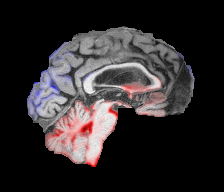
\includegraphics[height=2.5cm]{data/combined_sagittal.png}
            };

            \node[] at (0, 1) {
                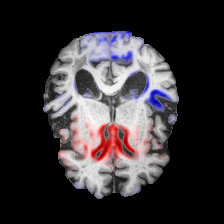
\includegraphics[height=2.5cm]{data/combined_axial.png}
            };

            \node[] at (3.25, 1) {
                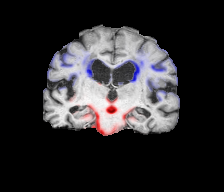
\includegraphics[height=2.5cm]{data/combined_coronal.png}
            };
            \node [
                left color=blue,
                right color=red,
                transform shape,
                draw=black,
                minimum height=0.25cm,
                text width=8cm,
            ] (colorbar) at (0, -1.5){};
            \node[font=\footnotesize\linespread{0.85}\selectfont, align=center, anchor=north] at (colorbar.south east) {
                Older\\appearing
            };
            \node[font=\footnotesize\linespread{0.85}\selectfont, align=center, anchor=north] at (colorbar.south west) {
                Younger\\appearing
            };
        }
        \visible<7>{
            \node[] at (0, 0) {
                \usebox{\patients}
            };
        }
        \visible<8>{
            \node[anchor=south] at (0, -3.5) {
                \usebox{\clinicalbaseline}
            };
        }\visible<9>{
            \node[anchor=south] at (0, -3.5) {
                \usebox{\clinicalbrainage}
            };
        }
        \visible<10>{
            \node[anchor=south] at (0, -3.5) {
                \usebox{\clinicalheatmaps}
            };
        }
    \end{tikzpicture}
\end{frame}
